\documentclass{article}
\usepackage[T1]{fontenc}
\usepackage[utf8]{inputenc}
\usepackage{lmodern}
\usepackage{textcomp}
\usepackage{geometry}
\usepackage{tikz}
\usepackage{pgfplots}
\usepackage{amsmath}
\pgfplotsset{compat=newest}
\geometry{
top=20mm,
bottom=25mm,
left=15mm,
right=15mm,}


\title{PAG 9.2\\\large The rate of reaction of calcium carbonate and hydrochloric acid}
\date{}
\author{Rosie Bartlett}

\begin{document}
\maketitle
\section{Mass experiment}
\subsection{Results}
\begin{center}
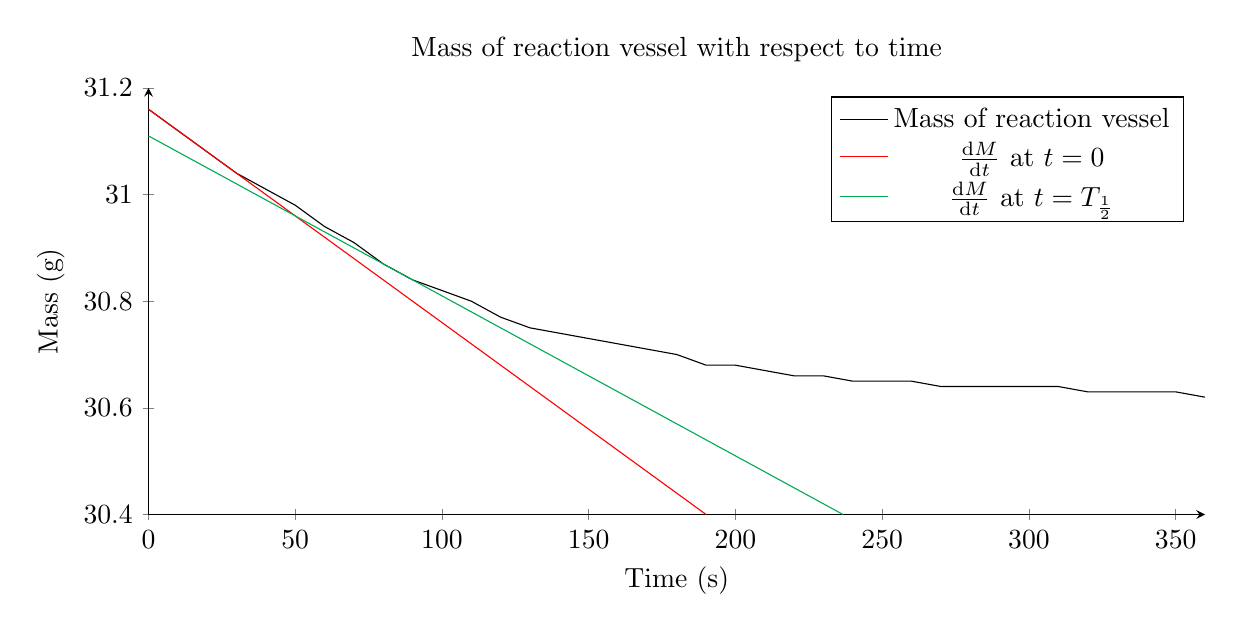
\begin{tikzpicture}
\begin{axis}[
axis lines=left,
clip=false,
samples=100,
xlabel=Time (s),
ylabel=Mass (g),
xmin=0,
xmax=360,
ymin=30.4,
ymax=31.2,
width=15cm,
height=7cm,
title=Mass of reaction vessel with respect to time]
\addplot[]
coordinates {(0, 31.16)
(10, 31.12)
(20, 31.08)
(30, 31.04)
(40, 31.01)
(50, 30.98)
(60, 30.94)
(70, 30.91)
(80, 30.87)
(90, 30.84)
(100, 30.82)
(110, 30.8)
(120, 30.77)
(130, 30.75)
(140, 30.74)
(150, 30.73)
(160, 30.72)
(170, 30.71)
(180, 30.7)
(190, 30.68)
(200, 30.68)
(210, 30.67)
(220, 30.66)
(230, 30.66)
(240, 30.65)
(250, 30.65)
(260, 30.65)
(270, 30.64)
(280, 30.64)
(290, 30.64)
(300, 30.64)
(310, 30.64)
(320, 30.63)
(330, 30.63)
(340, 30.63)
(350, 30.63)
(360, 30.62)
};
\addlegendentry{Mass of reaction vessel}
\addplot[color={rgb:red,255;green,0;blue,0}]
coordinates {(0, 31.16)
(190, 30.4)
};
\addlegendentry{$\frac{\mathrm{d}M}{\mathrm{d}t}$ at $t=0$}
\addplot[color={rgb:red,0;green,255;blue,125}]
coordinates {(0, 31.11)
(236.66666666666666, 30.4)
};
\addlegendentry{$\frac{\mathrm{d}M}{\mathrm{d}t}$ at $t=T_{\frac12}$}
\end{axis}
\end{tikzpicture}
\end{center}
\subsection{Analysis of results}
\begin{enumerate}
\item Half life 1 $\rightarrow$ 75s\\Half life 2 $\rightarrow$ 55s\\Half life 3 $\rightarrow$ 55s 

\item The half live values above include one anomaly, which when excluded give a constant half life. 

\end{enumerate}
\section{Gas reaction}
\subsection{Results}
By using the formula below, we can calculate the concentration of HCl from the volume of gas produced. Where $V(\text{CO}_2)$ is the volume of CO$_2$ produced. 
\begin{equation*}
[\text{HCl}]=\frac{120-V(\text{CO}_2)}{240}
\end{equation*}
\begin{center}
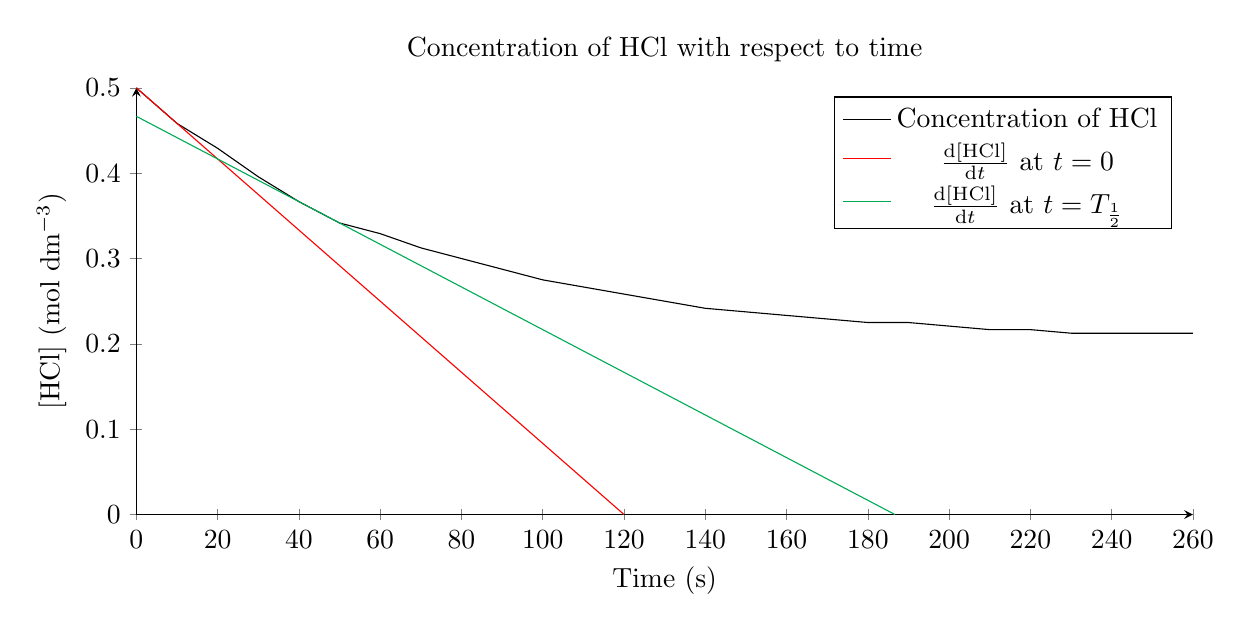
\begin{tikzpicture}
\begin{axis}[
axis lines=left,
clip=false,
samples=100,
xlabel=Time (s),
ylabel={[HCl]} (mol dm$^{-3}$),
xmin=0,
xmax=260,
ymin=0,
ymax=0.5,
width=15cm,
height=7cm,
title=Concentration of HCl with respect to time]
\addplot[]
coordinates {(0, 0.5)
(10, 0.45833)
(20, 0.42917)
(30, 0.39583)
(40, 0.36667)
(50, 0.34167)
(60, 0.32917)
(70, 0.3125)
(80, 0.3)
(90, 0.2875)
(100, 0.275)
(110, 0.26667)
(120, 0.25833)
(130, 0.25)
(140, 0.24167)
(150, 0.2375)
(160, 0.23333)
(170, 0.22917)
(180, 0.225)
(190, 0.225)
(200, 0.22083)
(210, 0.21667)
(220, 0.21667)
(230, 0.2125)
(240, 0.2125)
(250, 0.2125)
(260, 0.2125)
};
\addlegendentry{Concentration of HCl}
\addplot[color={rgb:red,255;green,0;blue,0}]
coordinates {(0, 0.5)
(120, 0)
};
\addlegendentry{$\frac{\mathrm{d}[\text{HCl}]}{\mathrm{d}t}$ at $t=0$}
\addplot[color={rgb:red,0;green,255;blue,125}]
coordinates {(0, 0.4666666666666667)
(186.66666666666666, 0)
};
\addlegendentry{$\frac{\mathrm{d}[\text{HCl}]}{\mathrm{d}t}$ at $t=T_\frac12$}
\end{axis}
\end{tikzpicture}
\end{center}
\subsection{Analysis of results}
\begin{enumerate}
\item Half life 1 $\rightarrow$ 43.5s\\Half life 2 $\rightarrow$ 50s\\Half life 3 $\rightarrow$ 45.5s 

\item Since all the half lives are similar, we can suggest that the reaction is first order. 

\end{enumerate}
\section{Extension opportunities}
\begin{enumerate}
\item \begin{enumerate}
\item Mass lost:\\Since there was an excess of CaCO$_3$, when the reaction reached completion, there would have been 0.04 mol of CO$_2$ produced. this would hav had a mass of 0.88g, meaning 0.88g would have been lost. In the reaction we only saw a loss of 0.5g, so the reaction did not go to completion.\\ Gas produced:\\Again the CaCO$_3$ was in excess, so at the end of the reaction, 0.01 mol of CO$_2$ would have been produced, with a volume of 120cm$^3$. we only saw a maximum volume of 69cm$^3$, so the reaction did not go to completion. 

\item As the reaction progresses, the concentration of HCl is constantly decreasing, which constantly decreases the rate, meaning a very long long time would be required to run the reaction to completion. 

\item For the reaction to go to completion, we would need a larger gas syringe to account for the extra 20cm3 of CO2 produced. 

\end{enumerate}

\item Mass lost:\\At $t=0$, $\frac{\mathrm{d}M}{\mathrm{d}t}$ was $-4\times10^{-3}$ g s$^{-1}$. At $t=T_\frac12$, $\frac{\mathrm{d}M}{\mathrm{d}t}$ was $-3\times10^{-3}$ g s$^{-1}$.\\ Gas produced:\\At $t=0$, $\frac{\mathrm{d}[\text{HCl}]}{\mathrm{d}t}$ was $\frac1{240}$ mol dm$^3$ s$^{-1}$ or approximately $4.17\times10^{-3}$ mol dm$^3$ s$^{-1}$. At $t=T_\frac12$, $\frac{\mathrm{d}[\text{HCl}]}{\mathrm{d}t}$ was $2.5\times10^{-3}$ mol dm$^3$ s$^{-1}$.\\ In both cases, the gradient at $T_\frac12$ is approximately half of what t was at $t=0$, giving further evidence that the reaction is first order. 

\end{enumerate}
\end{document}